\documentclass{scrartcl}

%%% Fonts and language setup.
\usepackage{polyglossia}
% Setup fonts.
\usepackage{fontspec}
\setmainfont{CMU Serif}
\setsansfont{CMU Sans Serif}
\setmonofont{CMU Typewriter Text}

\usepackage{microtype} % Add fancy-schmancy font tricks

%%% Polyglossia setup after (nearly) everything as described in documentation.
\setdefaultlanguage{russian}
\setotherlanguage{english}

\usepackage{csquotes}

%% Math
\usepackage{amsmath, amsfonts, amsthm, mathtools} % Advanced math tools.
% \usepackage{amssymb}

\usepackage{euler-math}

% \usepackage{unicode-math} % Allow TTF and OTF fonts in math and allow direct typing unicode math characters.
% \unimathsetup{
%     warnings-off={
%         mathtools-colon,
%         mathtools-overbracket
%         }
%     }

\usepackage{caption}

\NewDocumentCommand{\bone}{}{\mathbb{1}}
\NewDocumentCommand{\Ex}{}{\mathrm{Ex}}
\NewDocumentCommand{\CE}{}{\mathrm{CE}}
\NewDocumentCommand{\B}{}{B_{n \times n}}
\NewDocumentCommand{\C}{}{C_{n \times n}}
\NewDocumentCommand{\trace}{}{\mathrm{trace}}

%%% HyperRef
\usepackage{hyperref}

\title{Отчёт по лабораторной работе}
\subtitle{Файл: \texttt{labA\_01.cpp}}
\author{Н.А. Пономарев, группа 25.М71-мм}

\begin{document}

\maketitle

Некоторые обозначения, используемые в данном тексте:
\begin{itemize}
    \item $A_{m \times n} = (a_{ij})$~--- матрица из $m$ строк и $n$ столбцов, а $a_{ij}$~--- элемент матрицы на строке $i$, столбце $j$.
    \item $\bone_{m \times n}$~--- матрица из единиц, соответствующего размера.
    \item $E_{n \times n}$~--- единичная матрица.
    \item $\delta_{ij}$~--- символ Кронекера.
\end{itemize}

\section{Алгоритм}

Алгоритм вычисляет значение некоторого матричного выражения.
Все элементы матриц принадлежат полю вещественных чисел.
На вход алгоритм получает матрицы $\B$, $\C$, и векторы $x_{n \times 1}$, $y_{n \times 1}$.
В результате работы алгоритма получается матрица $A_{n \times n}$.

Первым делом вычисляется значение скаляра $\Ex$ по формуле:
\[
    \Ex = \sum_{i = 0}^{n - 1} x_i = \bone_{1 \times n} \cdot x_{n \times 1}.
\]
Фактически считаем скалярное произведение.

Затем вычисляется вектор $\CE_{n \times 1}$:
\[
    \CE = \C \cdot \bone_{n \times 1}
\]
или поэлементно:
\[
    \mathrm{ce}_{i1} = \sum_{i = 0}^{n - 1} c_{ik}.
\]
Фактически получаем вектор сумм строк.

Далее вычисляем скаляр $\trace$, который не является настоящим следом матрицы:
\[
    \trace = \sum_{i=0}^{n-1} \sum_{k=0}^{n-1} b_{ik} \cdot \mathrm{ce}_{k1} = \bone_{1 \times n} \cdot \B \cdot \CE_{n \times 1}.
\]

Затем вычисляем скаляр $z_1$:
\[
    z_1 = \sum_{i=0}^{n-1} \sum_{j=0}^{n-1} b_{ij} \cdot \Ex \cdot y_i = \Ex \cdot (y^\top)_{1 \times n} \cdot \B \cdot \bone_{n \times 1},
\]
скаляр $z_2$ (просто скалярное произведение):
\[
    z_2 = \sum_{i=0}^{n-1} x_i y_i = (x^\top)_{1 \times n} \cdot y_{n \times 1},
\]
и скаляр $z = z_1 / z_2$.

В конце формируем матрицу $A_{n \times n}$:
\[
    A = \trace \cdot \C + z \cdot \bone_{n \times n} + E_{n \times n}
\]
или поэлементно:
\[
    a_{ij} = \trace \cdot c_{ij} + z + \delta_{ij}.
\]

\paragraph{Обсуждение алгоритма.}
Сам по себе алгоритм б\'ольшую часть времени занимается свёртками и выглядит довольно сложным для распараллеливания, поскольку мало независимых операций и вероятно большая нагрузка на работу с памятью.

\section{Работа с кодом}

В процессе выполнения работы код был модифицирован следующим образом:

\begin{itemize}
    \item Исправлена синтаксическая ошибка в виде незакрытой фигурной скобки.
    \item Добавлен парсер аргументов командной строки.
    \item Слегка изменён вывод для упрощения постановки экспериментов.
    \item Декомпозирована логика вычислений для упрощения исследования и распараллеливания.
    \item Добавлен \textsc{CMake}.
    \item Применены исправления от \textsc{clang-format} и \textsc{clang-tidy}.
    \item Написан скрипт для проведения замеров.
\end{itemize}

\section{Исследования hotspot'ов}

С помощью утилит \textsc{perf} и \textsc{flamegraph}, был построен следующий график (см. рисунок~\ref{flamegraph}), приближенный внутрь функции \texttt{compute} (картинка векторная, можно приблизить):

\begin{figure}
    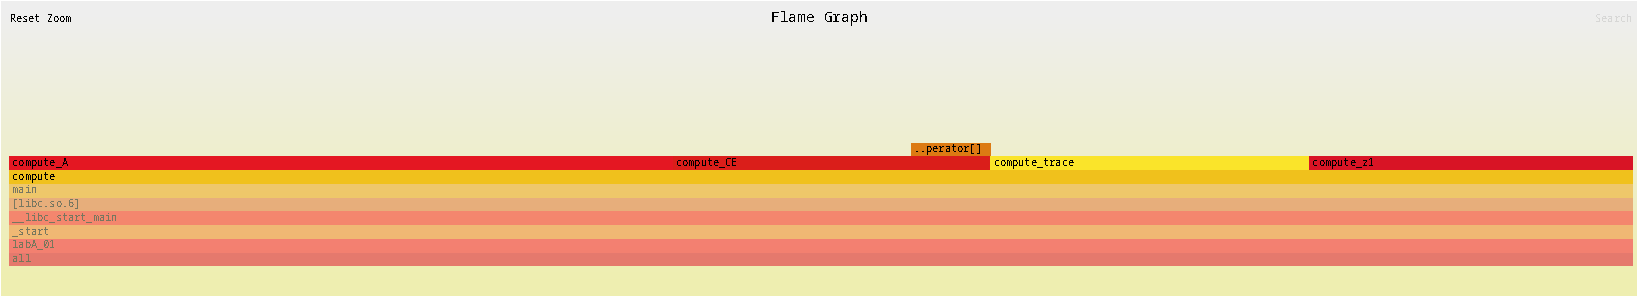
\includegraphics[width=\linewidth]{flamegraph.pdf}
    \caption{}
    \label{flamegraph}
\end{figure}

График, вероятно, подтверждает, что сложность алгоритма не в вычислениях, а в работе с памятью.

\section{Распараллеливание}

В соответствии с заданием, распараллеливание выполнялось с использованием двух технологий: \textsc{OpenMP} и \textsc{MPI (OpenMPI)}.

Поскольку алгоритм состоит в основном из операций свёртки, то циклы второго уровня вложенности специально не распараллеливались, поскольку по эмпирическим оценкам время на создание потока больше, чем время работы вложенных циклов.

\section{Исследование масштабируемости}


Измерения проводились на системе с процессором Intel(R) Xeon(R) E-2136 CPU @ 3.30GHz с 12 потоками.

В случае с \textsc{MPI} измерения на кластере произвести не удалось, поэтому кластером служил тот же многоядерный процессор.

Измерения проводились при фиксированном $n = 10\,000$ и изменяющемся количество потоков от 1 до максимальной степени двойки меньшей количеству потоков и с использованием всех потоков.

\begin{figure}
    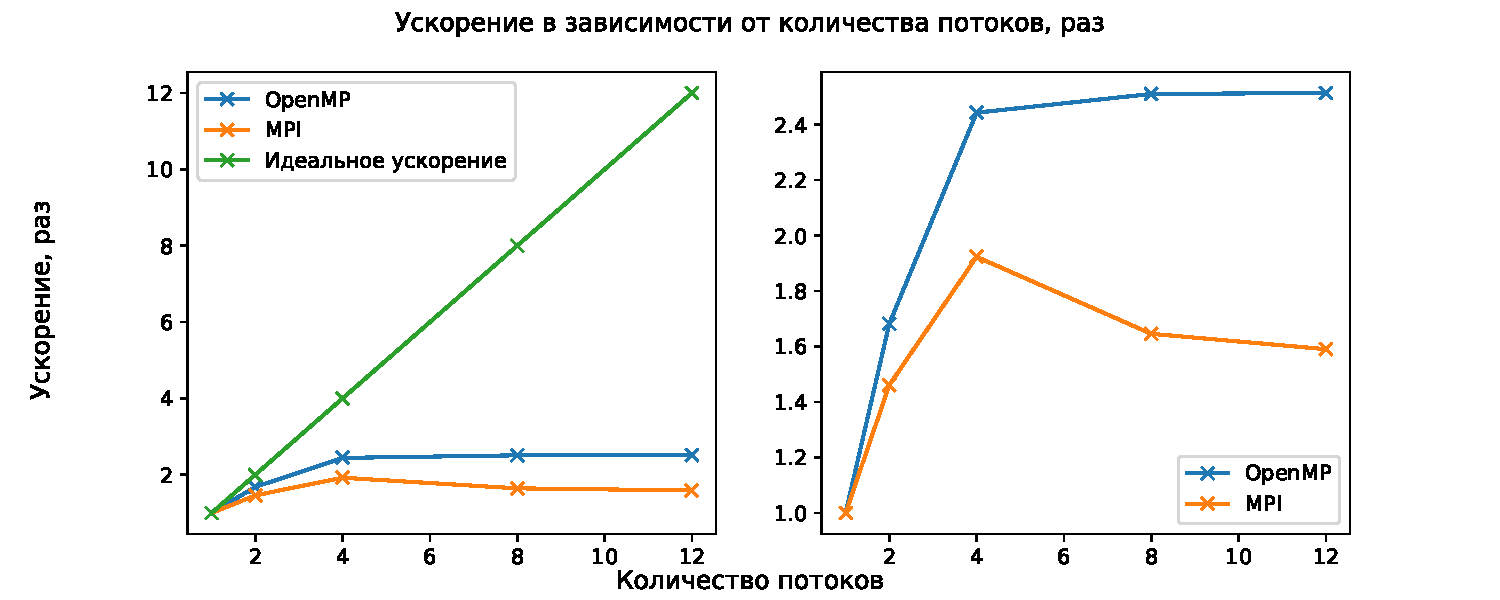
\includegraphics[width=\linewidth]{results.pdf}
    \caption{}
    \label{speedup}
\end{figure}

Перед запуском измерений при некотором фиксированном количестве ядер производилось 3 разогревочных запуска, затем производилось 10 измерений.

Итого, были получены результаты, изображенные на рисунке~\ref{speedup}.
Графики идентичны друг другу, отличие только в том, что на правом отсутствует график идеального распределения ради более детального анализа фактического ускорения.

\paragraph{Анализ ускорения.}
График показывает, что достичь идеального ускорения даже близко не получается.
Более того, в сравнению с 4 потоками, на 8 и 12 потоках в случае \textsc{OpenMP} прирост почти не наблюдается, а в случае \textsc{MPI} происходит замедление.
Полагаю, что это связано с тем, что затраты на обмен данными и создание потоков начинают сравниваться с временем вычислений для \textsc{OpenMP} и превышают затраты на вычисления в случае \textsc{MPI}.

\section*{Выводы}

В рамках лабораторной работы были выполнены следующий задачи:
\begin{enumerate}
    \item Проанализирован алгоритм.
    \item Улучшен код и создано окружение для сборки и измерений.
    \item Проведено распараллеливание с помощью \textsc{OpenMP} и \textsc{MPI (OpenMPI)}.
    \item Проведены и проанализированы эксперименты.
\end{enumerate}

К сожалению, большого ускорения достичь не удалось, что, вероятно, вызвано структурой самого алгоритма.

Исходный код доступен в репозитории: \url{https://github.com/WoWaster/spbu-hpc}.


\end{document}
